\chapter{REFERENCIAL TEÓRICO}

\section{Manufatura Aditiva}
O princípio básico por trás da manufatura aditiva (MA) é a 
capacidade de fabricar um modelo tridimensional diretamente, 
sem a necessidade de um planejamento do processo, a partir de 
um modelo tridimensional digital normalmente criado a partir 
de Computer Aided Design (CAD). Uma das características 
principais da MA é a rapidez na qual é possível criar protótipo
diretamente de modelos digitais, por conta disso, em um contexto 
de desenvolvimento de produto, o termo prototipagem rápida era 
utilizado. Entretanto, conforme a MA foi se aperfeiçoando era 
perceptível a capacidade dessas tecnologias não só se aterem à 
produção de protótipos, mas também de peças utilizadas em 
produtos finais. Além disso, o termo não considerava o princípio 
básico que unia essas tecnologias e assim o termo manufatura 
aditiva foi apresentado e adotado pela American Society for 
Testing and Materials (ASTM) \citeauthor{gibson15} (\citeyear{gibson15}).

Apesar da manufatura aditiva ter sido criada a mais de 30 anos, apenas
a partir de 2009, quando a última patente mais relevante de *Fused Deposition Modeling* (FDM)
expirou. Com isso, vários entusiastas começaram a desenvolver essa tecnologia de uma
maneira "caseira", com o forte movimento RepRap. Por conta dessa característica
"caseira" e um senso de comunidade, os desenvolvimentos em sua maioria eram
de caráter *Open Source* e com uma mentalidade de acessibilizar essa tecnologia para as pessoas.
Com os avanços tecnologicos feitos pela comunidade, empresas, pessoas e a mídia começaram
a se interessar cada vez mais, aumentando a popularidade das impressoras 3D e por consequência
trazendo muita atenção para a manufatura aditiva, que a partir dai, mais pesquisas, mais
empresas se interessavam em desenvolver esse tipo de tecnologia, não somente FDM \cite{attaran17}.

Atualmente, existe uma grande variedade de tecnologias e processos de manufatura aditiva.
Estes variam na maneira com que depositam o material, nos principios físicos que utilizam e nos materias
que podem ser utilizados. Como mencionado anteriormente, um dos métodos de manufatura aditiva mais populares
é a tecnologia FDM, entretanto existem diversas outras tecnologias que tem crescido muito em popularidade
como as tecnologias baseadas na cura seletiva de resinas, *stereolithography* (SLA) e *Masked stereolithography Apparatus* (MSLA),
alem de outras tecnologias menos acessíveis, mas com aplicações em diversas industrias, como por exemplo
*selective laser melting* (SLM) e *selective laser
sintering* (SLS) \cite{bikas16}.  

% \begin{figure}[!htb]
%     \centering
%     \caption{teste}
%     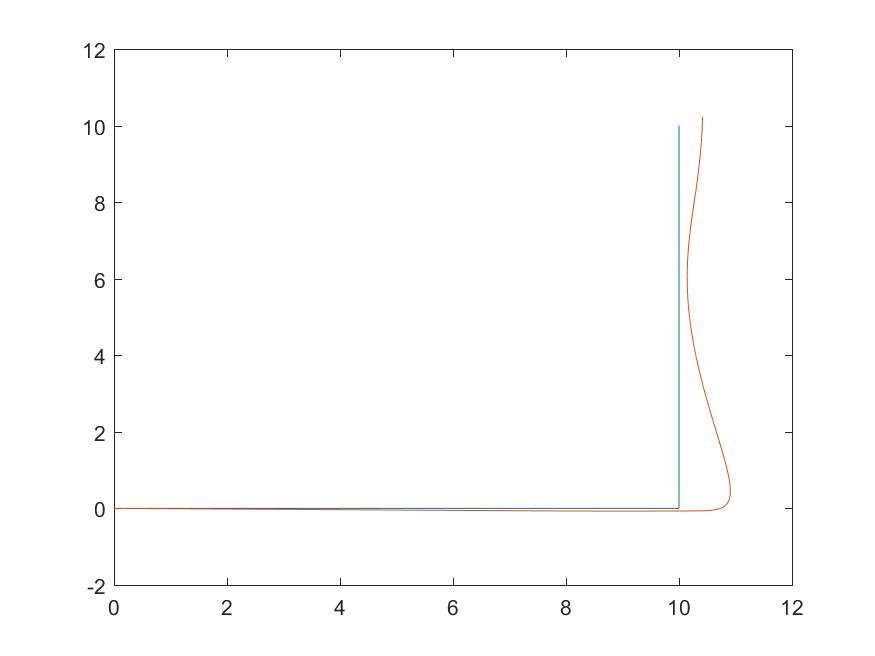
\includegraphics[scale=0.5]{Runge_kutta_comando_base_0001.jpg}
%     {\footnotesize Fonte: Elaborada pelo autor.}
%     \label{fig:label}
% \end{figure}

% \ref{fig:label} figura

\section{Fused Deposition Modeling}
Fused Deposition Modeling (FDM) ou Fused Filament Fabrication 
(FFF) é uma das tecnologias MA mais populares como mencionado anteriormente.
Ela se consiste por depositar material através de um processo 
onde um filamento de material é forçado dentro de uma câmara através,
geralmente, de rolos dentados onde em uma região específica esse 
material é liquefeito. Por conta da pressão criada pelo filamento 
adentrando a câmara, ainda no estado sólido como um pistão, 
o material liquefeito é extrudado através de um bocal, 
comumente fabricado de bronze. Então, o filamento liquefeito é 
depositado em uma plataforma de forma a percorrer a trajetória 
desejada utilizando mecanismos movidos de forma controlada, 
geralmente por motores de passos. O processo é repetido camada 
por camada, de forma que elas estejam apoiadas por camadas 
anteriores e a primeira camada continue fixa na plataforma ou 
cama, até que o processo finalize (TURNER et al., 2014) \cite{turner14}.

O trabalho de \cite{vyavahare20} apresenta algumas 
características sobre o desenvolvimento científico sobre 
FDM ao longo dos anos, tendo como base 211 artigos diferentes 
de 1994 a 2020. É apresentado um grande salto no número de 
artigos publicados no tema em anos recentes (2015 a 2018) 
(Figura 1), com 56\% dos temas trabalhados em torno da 
otimização de parâmetros de impressão, acompanhado de 17\% de 
trabalhos relacionados a aplicações utilizando o processo FDM, enquanto apenas x\%
são relacionados a outros temas, incluindo avanços tecnologicos relacionados
a melhorias de hardware e software desses dispositivos.
(Figura 2).

Podemos separar, de maneira simplificada, a porção de software de impressoras 3D
FDM em três principais etapas: fatiamento (slicing), geração de comando e controle.
A etapa de fatiamento involve a topologia e a criação de instruções a partir do modelo,
é nessa fase onde se decide a sequência de movimentos e outros eventos.
Já na etapa de geração de comando, as instruções criadas pelo fatiador (slicer) na etapa anterior
são interpretadas e os comandos detalhados são gerados, por exemplo as curvas de velocidade.
Esses comandos são utilizados para movimentar os motores e outros equipamentos da impressora.
Na etapa de controle, uma etapa relativamente nova nas impressoras 3D mais acessíveis, 
tecnicas de controle são utilizadas para se diminuir vibrações e variações indesejadas em quaisquer
parâmetros controlados, como a temperatura do bico. Um dos grandes avanços nessa etapa
foi a implementação da técnica de Input Shaping por um firmware Open Source de impressora 3D chamado Klipper.
Após a inclusão dessa etapa, principalmente no controle dinâmico da impressora, as capacidades
de velocidades e qualidade chegaram a outro patamar se comparados a impressoras que não implementam essa etapa \cite{klipperdoc}.

\subsection{5 Section S curve}

\subsection{Feedforward}
Dentre os métodos de controle em aplicações FDM o Feedforward 
é o mais eficiênte dada as limitações de custo em impressoras 
3D comuns e é capaz de ter um impacto maior em sistemas 
conhecidos e sensíveis ao erro, onde buscam corrigir o erro 
antes que ele aconteça \cite{ramani20,duan18}.

texto

\subsubsection{Input Shaper}
Conhecendo a trajetória desejada e conhecendo características 
do sistema é possível computar os comandos fornecidos para 
calcular uma série de comandos, levando em consideração as 
características do sistema para que o comando de referência 
seja modificado de forma à trajetória final ser o mais próximo 
possível do comando de referência. Entretanto, ao invés de 
computar todo o comando de referência, é possível obter um 
comando modificado em tempo real através de um filtro. 
Uma das abordagens desse tipo de filtro de comando é o 
Input Shaper, onde variados Shapers são construídos levando 
em consideração diferentes objetivos e restrições 
\cite{singhose97}.
Essa abordagem vem sendo utilizada na comunidade Maker depois 
da patente ter perdido o vigor, e tem aprimorado a área como
um todo, empurrando os limites anteriores de velocidade e 
precisão.

\subsubsection{B-spline}
texo
\subsubsection{Robust Filter}
texto




\section{Geração de comando}
A geração de comando é o processo que coordena a ativação dos 
atuadores, motores, dentre outros componentes de uma impressora. 
Ele recebe como base uma série de comandos que precisam ser 
interpretados e interpolados. Esse processo é responsável pelo 
controle de velocidade, aceleração dentre outras atividades que 
variam no tempo. O desenvolvimento científico nesta área 
aplicado a impressoras 3D FDM se deu em tempos recentes, 
sendo sua aplicação majoritária relacionada às máquinas de 
Controle Numérico Computadorizado (CNC).

\subsection{Look ahead}
No processo de impressão 3D são fornecidos para a impressora 
uma sequência de pontos no espaço e limitações de velocidade 
entre os mesmos. A velocidade nos pontos é compartilhada entre 
trajetos em sequência, o que torna considerá-los 
independentemente ineficiente, introduzindo aceleração e 
desaceleração desnecessária impactando negativamente no tempo 
de impressão e na qualidade da peça impressa.
O algoritmo Look Ahead procura manter o máximo de velocidade 
possível entre movimentos distintos, evitando acelerações e 
desacelerações desnecessárias, apesar de ser necessário um 
pré-processamento desses pontos que introduzem um custo 
computacional maior (YU et al. 2020) \cite{yu20, klipperkinematic}.

Para a construção da curva de velocidade trapezoidal a partir da matriz de posições
e *feedrate* é necessário o calculo das direções dos movimentos a serem realizados.

As direções são representadas por vetores unitários calculados a partir
do vetor deslocamento dividido pelo mesmo vetor normalizado. Sendo o vetor deslocamento
obtido pela diferença entre dois vetores de posição sequenciais.

Essas direções são utilizadas para o cálculo das velocidades pelo *look ahead*,
considerando os valores de desvio de junta como  0.1 e aceleração maxima de $5000 mm/s^2$

Calculamos então a velocidade de junção baseada no angulo das direções do movimento e
nos parâmetros da aceleração máxima e desvio máximo de junção.

Velocidade de cruzamento

equações


\subsection{Curvas de velocidade trapezoidal}
Trapezoidal, S shape, etc

equações


A partir dessa matriz de posições e, agora também velocidades,
utilizamos a função responsável por gerar a curva trapezoidal de velocidades.

Essa função separa o deslocamento total do movimento em 3 ou 2 fases de aceleração constante.
É utilizado a equação x para o cálculo da velocidade pico

A partir da comparação da velocidade pico com a velocidade desejada pelo *feedrate*.
Caso a velocidade de pico for maior do que a velocidade desejada, temos 3 fases de deslocamento
que são calculadas pelas equações x,x e x
Caso a velocidade de pico seja igual ou menor do que a velocidade desejada, teremos 2 fases de deslocamento
que são calculadas a partir das equações x e x.

Como resultado da função, obtemos uma nova matriz esta contendo informações
sobre o a variação da posição, do tempo, da velocidade e sobre a aceleração e direção de deslocamento no ponto.

A partir dessa matriz, utilizamos a função de interpolação para dividir cada intervalo dessa matriz em intervalos menores
baseados em uma configuração de passo de interpolação, no caso baseado em passos de tempo.
Assim criando-se uma nova matriz dos dados interpolados.

A partir dos vetores de direção e da função acumuladora que se consite em acumular os valores de um vetor.
Obtemos uma matriz de posições, velocidades e tempo.




\section{Modelagem e Controle}

texto

\subsection{Espaço de Estados}
texto

equações

\subsection{Modelagem dinâmica impressora 3D}

Para a modelagem dinâmica dos eixos X e Y da impressora 3D, 
é considerado que os eixos são completamente independentes, 
a flexibilidade da correia é aproximada utilizando um conjunto 
mola amortecedor e a transmissão de movimento e torque dos 
motores é considerada como ideal e não será abordada.
Assim duas posições de estudo surgem para cada eixo, uma delas 
representa a posição ideal e desejada pelo usuário (X1) e a 
segunda é a posição real considerando as forças inerciais e a 
flexibilidade introduzida pela correia (X2) como na Figura 4.

\subsection{Integradores numéricos}

texto


\subsubsection{Runge Kutta}
texto
equações


\subsection{Objective Function Optimization}
texto

\section{Matlab}

\subsection{fmincon}

Como o modelo matemático a ser otimizado é multivariável e 
possuindo restrições não-lineares, a função FMINCON do ambiente 
do MATLAB é utilizada para otimizar as variações de velocidade 
de forma a diminuir o erro de trajetória associado às 
flexibilidades do sistema que causam perturbações e vibrações 
indesejadas.
É uma função baseada em gradientes que busca por todos os 
mínimos locais de uma região que satisfaz outras restrições 
estipuladas \cite{albaghdadi21}.
Ela utiliza um conjunto de restrições superiores e inferiores 
para cada ponto e otimiza a função considerando as restrições 
estabelecidas pela função não linear, utilizando as equações de 
movimento para encontrar a resolução da EDO de maneira e 
otimizar os parâmetros utilizando o algoritmo sqp, com o 
objetivo de minimizar a seguinte função:


